
\documentclass[
	% -- opções da classe memoir --
	12pt,				% tamanho da fonte
	openright,			% capítulos começam em pág ímpar (insere página vazia caso preciso)
	twoside,			% para impressão em recto e verso. Oposto a oneside
	a4paper,			% tamanho do papel. 
	english,			% idioma adicional para hifenização
	french,				% idioma adicional para hifenização
	spanish,			% idioma adicional para hifenização
	brazil				% o último idioma é o principal do documento
	]{abntex2}

% ---
% Pacotes básicos 
% ---
\usepackage{mathptmx}			% Usa a fonte Latin Modern
\usepackage[T1]{fontenc}		% Selecao de codigos de fonte.
\usepackage[utf8]{inputenc}		% Codificacao do documento (conversão automática dos acentos)
\usepackage{indentfirst}		% Indenta o primeiro parágrafo de cada seção.
\usepackage{color}				% Controle das cores
\usepackage{graphicx}			% Inclusão de gráficos
\usepackage{microtype} 		% para melhorias de justificação
%\usepackage{subfig}
\usepackage[font=small]{caption}
\usepackage{setspace}
\captionsetup{justification=raggedright,singlelinecheck=false}
\usepackage[top=3cm, bottom=2cm, inner=3.5cm, outer=2cm]{geometry}
% ---
\usepackage{adjustbox}
\usepackage{amssymb}
\usepackage{amsmath}
\usepackage{tikz}
\usetikzlibrary{shapes,arrows}
\usepackage{extarrows}
\usepackage{braket}
\usepackage{subcaption}

\usepackage{fancyhdr}%Pacote para mudar o cabeçalho das páginas.

% ---
\usepackage{multirow}
\usepackage{textcomp}
% Pacotes adicionais, usados apenas no âmbito do Modelo Canônico do abnteX2
% ---
\usepackage{lipsum}				% para geração de dummy text
% ---

% ---
% Pacotes de citações
% ---
%\usepackage[brazilian,hyperpageref]{backref}	 % Paginas com as citações na bibl
\usepackage[alf]{abntex2cite}	% Citações padrão ABNT
\usepackage{fancyhdr}
\fancyhf{}
% --- 
% CONFIGURAÇÕES DE PACOTES
% --- 
\graphicspath{{./Figuras/}} 

\titulo{Modelo de dissertação da EEL}
\autor{Thiago Trevizam Dorini}
\local{Lorena}
\data{Ano}
%\orientador{Prof. Dr. Luiz Tadeu Fernandes Eleno}
%\coorientador{Prof. Dr. Gilberto Carvalho Coelho}
\instituicao{%
  Versão original}
\tipotrabalho{Dissertação (Mestrado)}
% O preambulo deve conter o tipo do trabalho, o objetivo, 
% o nome da instituição e a área de concentração 
\preambulo{
	\fontsize{12}{12}\selectfont
	Dissertação apresentado à Escola de Engenharia de Lorena da Universidade de São Paulo para a obtenção do título de Mestre em Ciências do Programa de Pós-Graduação em Engenharia de Materiais na area de Materiais Convencionais e Avançados.
	\newline
	\newline
	Orientador: Prof. Dr. Fulano de tal
}

\definecolor{blue}{RGB}{41,5,195}

% informações do PDF
\makeatletter
\hypersetup{
     	%pageref=true,
		pdftitle={\@title}, 
		pdfauthor={\@author},
    	pdfsubject={\imprimirpreambulo},
	    pdfcreator={LaTeX with abnTeX2},
		pdfkeywords={abnt}{latex}{abntex}{abntex2}{trabalho acadêmico}, 
		colorlinks=true,       		% false: boxed links; true: colored links
    	linkcolor=black,          	% color of internal links
    	citecolor=black,        		% color of links to bibliography
    	filecolor=magenta,      		% color of file links
		urlcolor=black,
		bookmarksdepth=4
}
\makeatother
% --- 

\makeatletter
\setlength{\@fptop}{5pt} % Set distance from top of page to first float
\makeatother
% ---

\newcommand{\quadroname}{Quadro}
\newcommand{\listofquadrosname}{Lista de quadros}

\newfloat[chapter]{quadro}{loq}{\quadroname}
\newlistof{listofquadros}{loq}{\listofquadrosname}
\newlistentry{quadro}{loq}{0}

% configurações para atender às regras da ABNT
\setfloatadjustment{quadro}{\centering}
\counterwithout{quadro}{chapter}
\renewcommand{\cftquadroname}{\quadroname\space} 
\renewcommand*{\cftquadroaftersnum}{\hfill--\hfill}

\setfloatlocations{quadro}{hbtp} % Ver https://github.com/abntex/abntex2/issues/176

\setlength{\parindent}{1.3cm}

% Controle do espaçamento entre um parágrafo e outro:
\setlength{\parskip}{0.2cm}  % tente também \onelineskip

% ---
% compila o indice
% ---
\makeindex
% ---

% ----
% Início do documento
% ----
\begin{document}

\selectlanguage{brazil}

% Retira espaço extra obsoleto entre as frases.
\frenchspacing 

% ---
\imprimirfolhaderosto*


\begin{fichacatalografica}
	\sffamily
	\vspace*{\fill}					% Posição vertical
	\begin{center}					% Minipage Centralizado
	\fbox{\begin{minipage}[c][8cm]{13.5cm}		% Largura
	\small
	\imprimirautor
	%Sobrenome, Nome do autor
	
	\hspace{0.5cm} \imprimirtitulo  / \imprimirautor. --
	\imprimirlocal, \imprimirdata-
	
	\hspace{0.5cm} \thelastpage p. : il. (algumas color.) ; 30 cm.\\
	
	\hspace{0.5cm} \imprimirorientadorRotulo~\imprimirorientador\\
	
	\hspace{0.5cm}
	\parbox[t]{\textwidth}{\imprimirtipotrabalho~--~\imprimirinstituicao,
	\imprimirdata.}\\
	
	\hspace{0.5cm}
		1. Palavra-chave1.
		2. Palavra-chave2.
		2. Palavra-chave3.
		I. Orientador.
		II. Universidade xxx.
		III. Faculdade de xxx.
		IV. Título 			
	\end{minipage}}
	\end{center}
\end{fichacatalografica}
% ---

\newpage
\begin{dedicatoria}
   \vspace*{\fill}
   \centering
   \noindent
   \textit{Espero que este template ajude nas monografias e dissertações dos alunos da EEL.} \vspace*{\fill}
\end{dedicatoria}
% ---

% ---
% Agradecimentos
% ---
\begin{agradecimentos}
	
	

\end{agradecimentos}
% ---

% ---
% Epígrafe
% ---
\begin{epigrafe}
    \vspace*{\fill}
	\begin{flushright}
		\textit{Acreditar em nossa própria mentira é o primeiro passo\\
		para o estabelecimento de uma nova verdade.\\
    (Carlos Drummond de Andrade)	}
	\end{flushright}
\end{epigrafe}
% ---

% ---
% RESUMOS
% ---

% resumo em português
\setlength{\absparsep}{18pt} % ajusta o espaçamento dos parágrafos do resumo
\begin{resumo}[RESUMO]
	
\'ULTIMO SOBRENOME, T. T. \textbf{Título do trabalho}. Ano. Número de páginas (Ex: 85p.) Dissertação (Mestrado em Ciências) - Escola de Engenharia de Lorena, Universidade de São Paulo, Lorena, 2019.

Faça um resumo do seu trabalho com uma pequena introdução, o objetivo a ser alcançado, uma breve descrição dos resultados, e termine com a conclusão.

 \textbf{Palavras-chave}: Colocar umas 7 palavras chaves. Chave 2. Chave 3. Chave 4, Chave 5, Chave 6.
 
 
\end{resumo}

% resumo em inglês
\begin{resumo}[ABSTRACT]
 \begin{otherlanguage*}{english}
 	
\'ULTIMO SOBRENOME, T. T. \textbf{Título do trabalho em inglês}. Ano. Páginas p. Dissertation (Master of Science). Escola de Engenharia de Lorena, Universidade de São Paulo, Lorena, 2019.

Pratique seu inglês! Tente não usar o google tradutor. Ou use, ninguém vai perceber mesmo.
 
   \noindent 
   \textbf{Keywords}: Palavras-chave em inglês.
     
 \end{otherlanguage*}
\end{resumo}
  
% ---

% ---
% inserir lista de ilustrações
% ---
\pdfbookmark[0]{\listfigurename}{lof}
\listoffigures*
\cleardoublepage
% ---

% ---
% inserir lista de tabelas
% ---
\pdfbookmark[0]{\listtablename}{lot}
\listoftables*
\cleardoublepage
% ---

\begin{siglas}
	\item[PGM] \textit{Platinum Group Metal}
	\item[TBC] \textit{Thermal Barrier Coating}
	
\end{siglas}
%\addcontentsline{toc}{chapter}{Lista de abreviaturas e siglas}

% ---

% ---
% inserir lista de símbolos
% ---

\begin{simbolos}
	
	\item[$ \Delta_fH$ ] Entalpia de formação
	\item[$ \hat{H} $] Operador Hamiltoniano
	\item[E] Autovalor de um operador do tipo hamiltoniano
	\item[$ \Psi $] Função de onda, autofunção do operador $\hat{H}$ com autovalor E
	
\end{simbolos}
% ---
\pdfbookmark[0]{\contentsname}{toc}
\tableofcontents*
\cleardoublepage
% ---
%\addcontentsline{toc}{chapter}{Lista de símbolos}

% ---


% ----------------------------------------------------------
% ELEMENTOS TEXTUAIS
% ----------------------------------------------------------
\textual

\pagestyle{fancy} %Estilo das páginas usando o pacote fancy.
\fancyhead[EL,OR]{\thepage} %O número das páginas pares (even E) fica à esqueda (left L), enquanto que das páginas ímpares (odd O) fica à direita (right R).
\renewcommand{\headrulewidth}{0pt} %Linha embaixo do número da página com espessura 0.

\chapter{Introdução}

Os alunos sempre acabam perdendo muito tempo somente formatando suas monografias e dissertações nos padrões malucos da ABNT e da EEL. Digo este 'e' porque a formatação da EEL usa somente em parte as normas da ABNT (vai entender porque), e pra descobrir quando usar uma ou outra pode ser trabalhoso e até estressante. Como já passei por isto, decidi usar a minha dissertação de mestrado como modelo, nos padrões que foram aceitos na biblioteca da EEL, com a intenção de ajudar os futuros alunos com suas respectivas dissertações ou monografias. 

Este template não aborda todos os padrões, somente os que foram mais essenciais que eu acabei usando. Não acredito que seja necessário usar muito mais do que há neste modelo, mas sintam-se a vontade para atualizar este documento, este é somente o ponto de partida. 

Os pacotes de formatação já estão todos adicionados, basta colocar o seu texto, figuras e tabelas nos locais apropriados e ser feliz! 

\begin{figure}
	\centering
	\caption{Exemplo de uma figura.}
	
\includegraphics[width=0.6\textwidth]{Got}
	\label{Selecione_um_label_para_chamar_no_texto_com_o_comando_ref{}.}
	\raggedright
	\caption*{Fonte: adaptado de Fullretard}
\end{figure}


\begin{figure}
	\centering
	\caption{Exemplo de figuras lado a lado.}
	\begin{subfigure}[t]{0.5\textwidth}
		\caption{Wolverine}
		\centering
		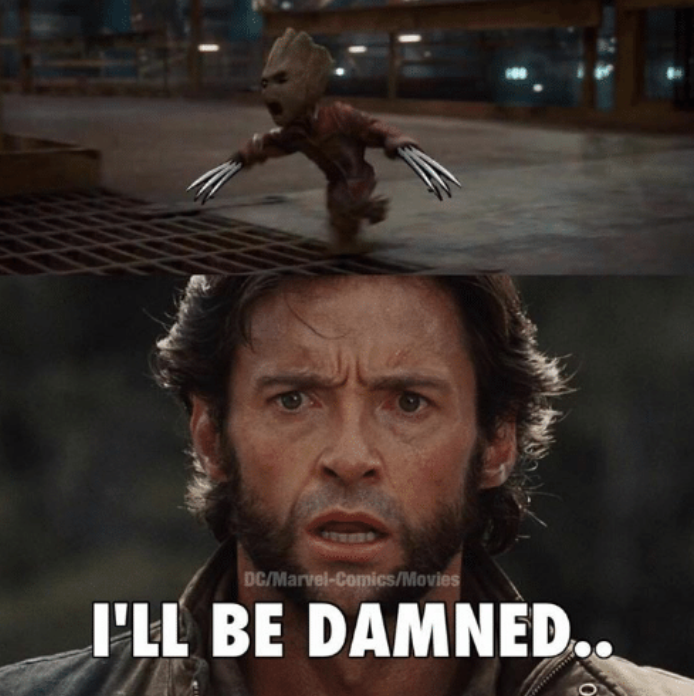
\includegraphics[width=\linewidth]{Wolverine}
	\end{subfigure}%\hskip 1em%
	\begin{subfigure}[t]{0.5\textwidth}
		\caption{Marvel}
		\centering
		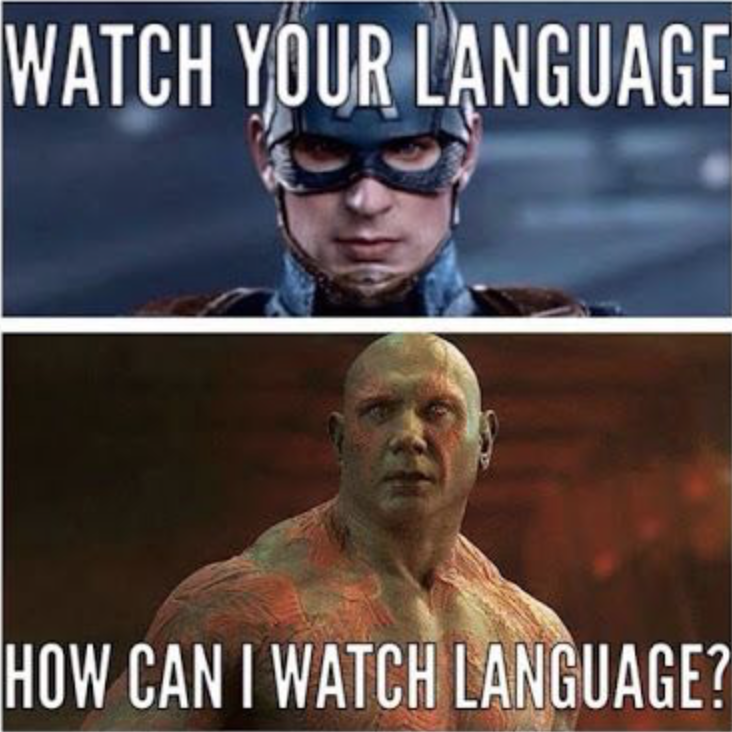
\includegraphics[width=\linewidth]{Drax}
	\end{subfigure}
	\begin{subfigure}[t]{0.5\textwidth}
		\caption{Dark Knight}
		\centering
		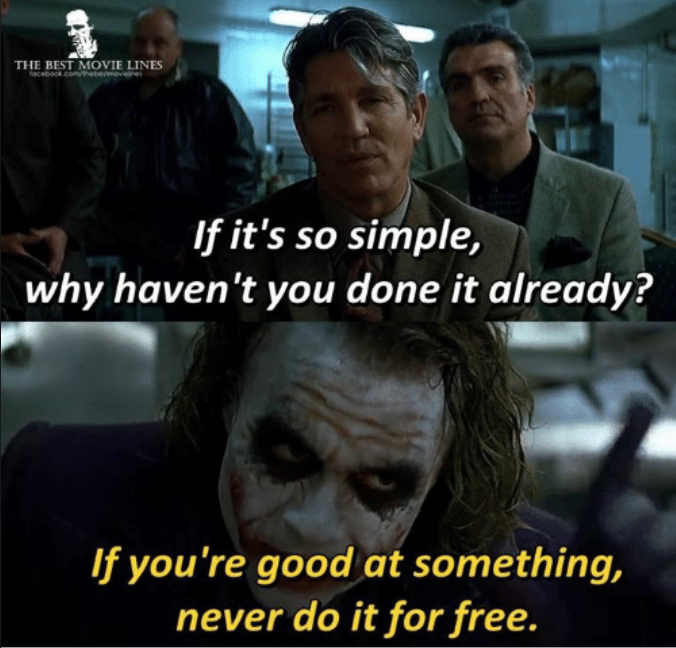
\includegraphics[width=\linewidth]{Coringa}
	\end{subfigure}%\hskip 1em%
	\begin{subfigure}[t]{0.5\textwidth}
		\caption{Interstellar}
		\centering
		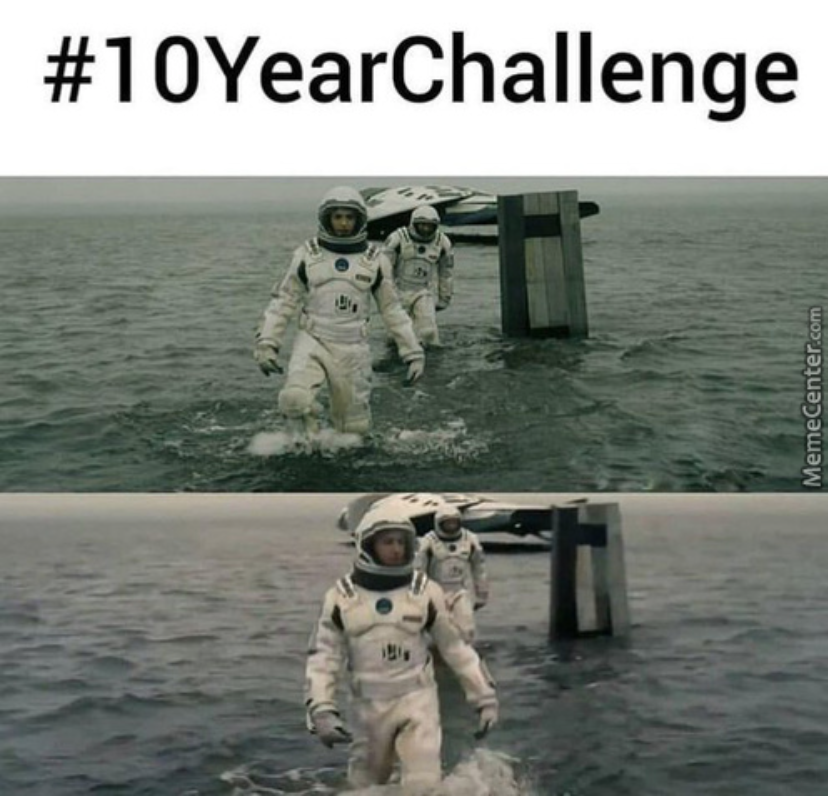
\includegraphics[width=\linewidth]{Interstelar}
	\end{subfigure}
	
	\begin{subfigure}[t]{0.5\textwidth}
		\caption{Inception}
		\centering
		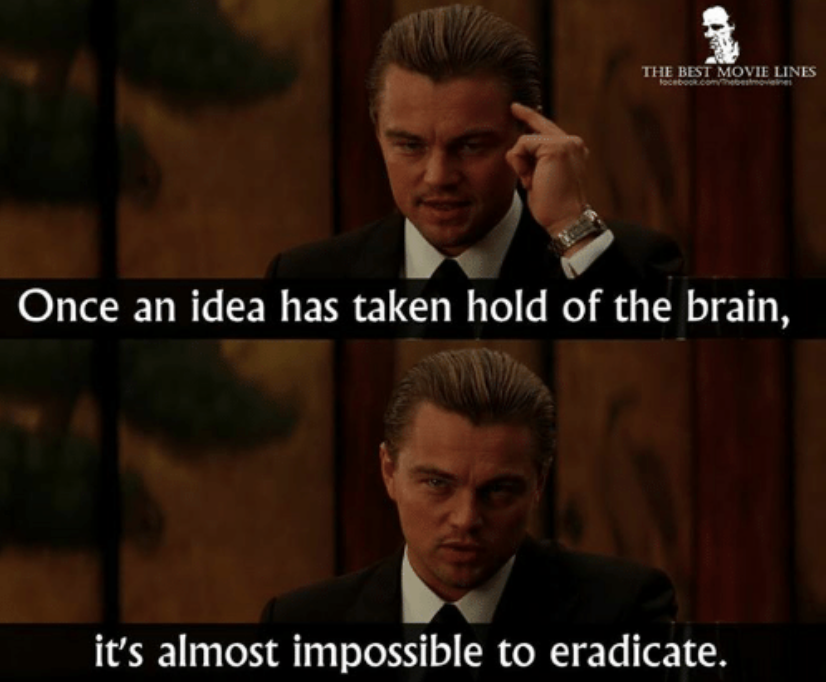
\includegraphics[width=\linewidth]{Leo}
	\end{subfigure}%\hskip 1em%
	\begin{subfigure}[t]{0.5\textwidth}
		\caption{The hateful eight}
		\centering		
		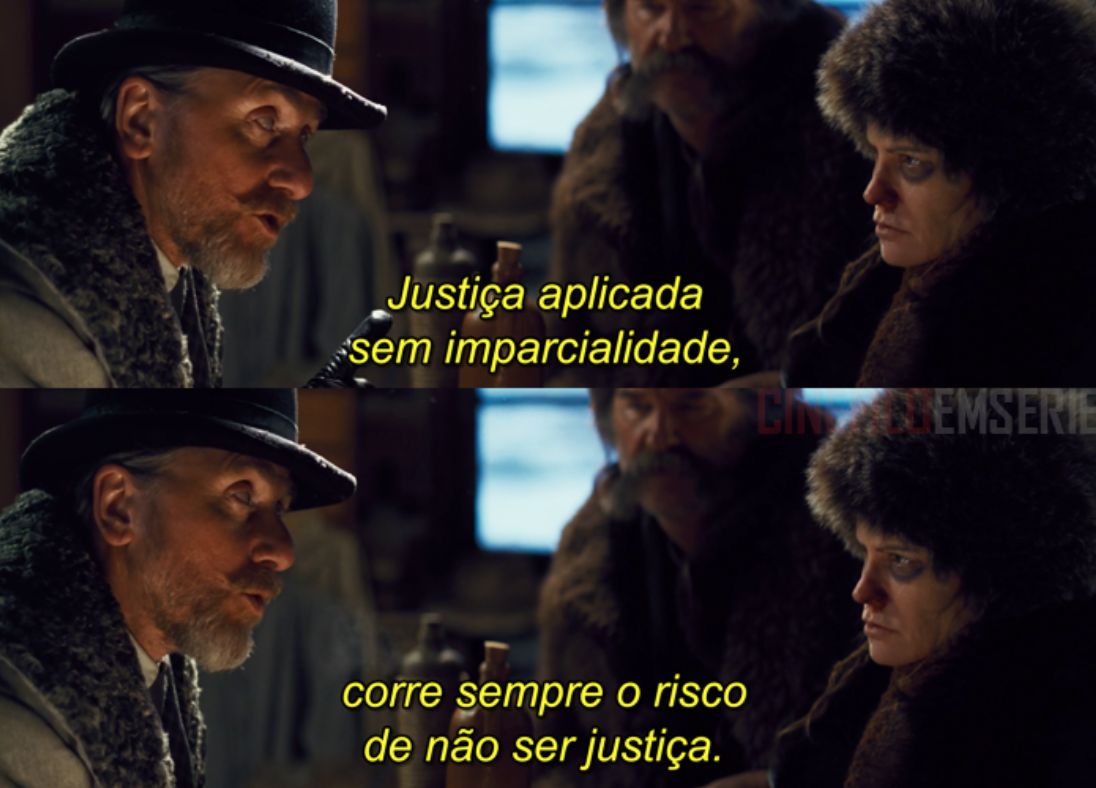
\includegraphics[width=\linewidth]{Odiados}
	\end{subfigure}
	\label{fig:mev1}
	\caption*{Fonte: autor}
	\caption*{Nota: Memes de filmes que valem a pena assistir.}
\end{figure}

\begin{table}
	\centering
	\caption{Exemplo de tabela com referências.}
	\begin{tabular}{ccc}
		\toprule
		Referências & $\Delta_f$H & Método\\
		\midrule
		\cite{Kleppa1998} & -33,6 & Calorimetria de síntese\\
		\cite{Eremenko1972} & -34,4 & Extrapolação (EMF)\\
		\cite{Lukashenko1986} & -34,8 & Extrapolação (EMF)\\
		\cite{Chart1975} & -27,9 & Efusão de Knudsen\\
		\cite{deBoer1982} & -31,0 & Estimativa (Miedema)\\
		\cite{Coughanowr1994} & -32,5 & Calculado (CALPHAD)\\
		\cite{Schuster2000} & -32,5 & Calculado (CALPHAD)\\
		\bottomrule
		
	\end{tabular}
	\label{tab:T1-entalpias}
	\caption*{Fonte: autor}
\end{table}

Equação simples:

\begin{equation}
\centering
\hat{H}\psi=E\psi
\label{Schro}
\end{equation}

Equação mais complicada:

\begin{multline}
\bigg[\overbrace{-\frac{\hbar}{2m_{i}}\sum_i\nabla_i^2}^{\hat{T}} +\overbrace{\frac{e^2}{4\pi\epsilon_0}\sum_j\sum_{j'>j}\frac{Z_jZ_{j'}}{|\vec{R}_j-\vec{R}_{j'}|}}^{\hat{V}_{NN}} -\overbrace{\frac{e^2}{4\pi\epsilon_0}\sum_i\sum_{j}\frac{Z_j}{|\vec{r}_i-\vec{R}_{j}|}}^{\hat{V}_{eN}} \\ +\underbrace{\frac{e^2}{4\pi\epsilon_0}\sum_i\sum_{i'>i}\frac{1}{|\vec{r}_i-\vec{r}_{i'}|}}_{\hat{V}_{ee}}\bigg]\Psi = E_{tot}\Psi
\end{multline}

\begin{figure}[h]
	\centering
	\caption{Exemplo do pacote tikz.}
	\tikzstyle{decision} = [diamond, draw, text width=7em, text centered, node distance=5cm, inner sep=0pt]
	\tikzstyle{block} = [rectangle, draw, text width=9em, text centered, rounded corners, minimum height=4em]
	\tikzstyle{line} = [draw, -latex']
	\begin{tikzpicture}[node distance = 5cm, auto]
	\node [block] (init) {Densidade inicial (estimativa) $\rho(\vec{r})$};
	\node [block, right of = init] (Kohn-Sham) {Resolver as equações de Kohn-Sham};
	\node[right of = Kohn-Sham] (step) {};
	\node [block, below of = step] (Electron-Density) {Energia $E$, nova densidade $\rho(\vec r)$};
	\node [decision, left of = Electron-Density] (Erro) {Energia convergiu?};
	\node [block, left  of = Erro] (convergido) {$E$ e $\rho(\vec{r})$ finais};
	\path [line] (init) -- (Kohn-Sham);
	\path [line] (Kohn-Sham) -| (Electron-Density);
	\path [line] (Electron-Density) -- (Erro);
	\path [line] (Erro) -- node {não} (Kohn-Sham);
	\path [line] (Erro) -- node {sim} (convergido);
	\end{tikzpicture}
	\label{SCF}\\
	\caption*{Fonte: \cite{Dorini2017}}
\end{figure}

\begin{figure}
	\centering
	\caption{Exemplo da aplicação do pacote \textit{minipage}.}
	\begin{minipage}{.4\textwidth}
		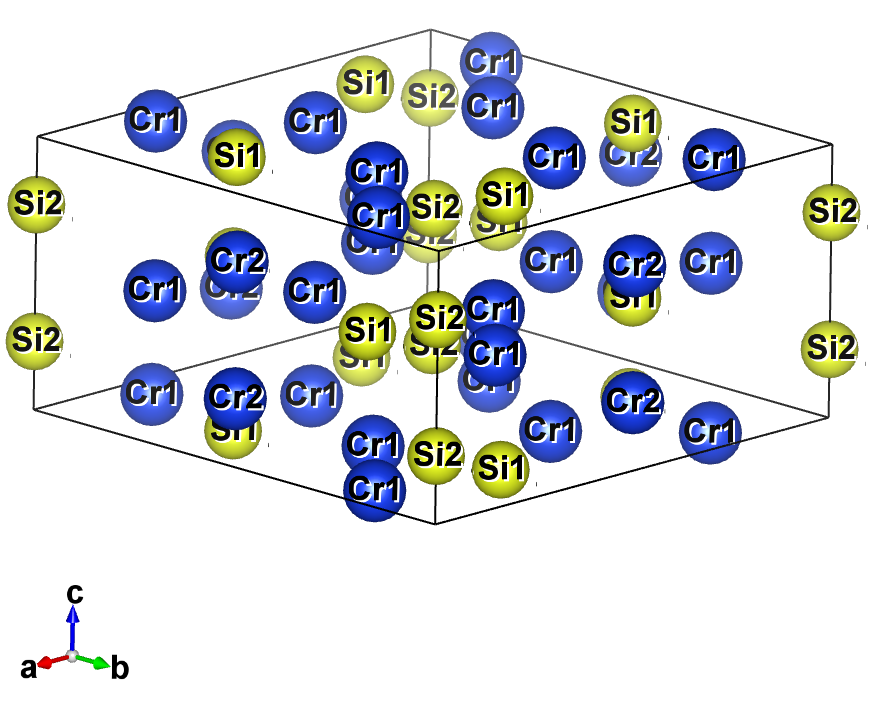
\includegraphics[width=\textwidth]{T1}
	\end{minipage}
	\begin{minipage}{.5\textwidth}
		\begin{tabular}{ll}
			%            Composto: & $\alpha$Cr$_5$Si$_3$ \\
			Grupo espacial: & $I4/mcm$ (\#140)\\
			Símbolo de Pearson: & $tI32$\\
			Protótipo: & W$_5$Si$_3$\\
			Parâmetros de rede: & $a=b=9,14\,$\AA ;  $c=4,64\,$\AA \\
			%            Posições atômicas:
		\end{tabular} \\
		% 
		\begin{tabular}{ccccccc}
			\toprule
			& Sítio & Wyckoff & Sim. & $x$ & $y$ & $z$     \\
			\midrule
			\tikz\draw[black,fill=blue!70] (0,0) circle (.7ex); & Cr1 & $16k$ & $m..$ & 0,074 & 0,223 & 0 \\
			\tikz\draw[black,fill=blue!70] (0,0) circle (.7ex); & Cr2 & $4b$ & $-42m$ & $0$ & $1/2$ & $1/4$ \\
			\tikz\draw[black,fill=yellow!70] (0,0) circle (.7ex); & Si1 & $8h$ & $m.2m$ & 0,17 & 0,67 & 0 \\
			\tikz\draw[black,fill=yellow!70] (0,0) circle (.7ex); & Si2 & $4a$ & $422$ & $0$ & $0$ & $1/4$ \\
			\bottomrule
		\end{tabular}
		%         (Hf: cinza claro; V: branco; Ga: cinza escuro)
	\end{minipage}
	\label{estrutura-T1}\\
	\caption*{Fonte: autor}
	\caption*{Nota: Adaptado de \cite{Kuzma1982}}
\end{figure}

\begin{figure}
	\centering
	\caption{Exemplo do pacote \textit{subfig} para ajustar duas figuras lado a lado.}
	\begin{subfigure}[t]{0.5\textwidth}
		\caption{}
		\centering
		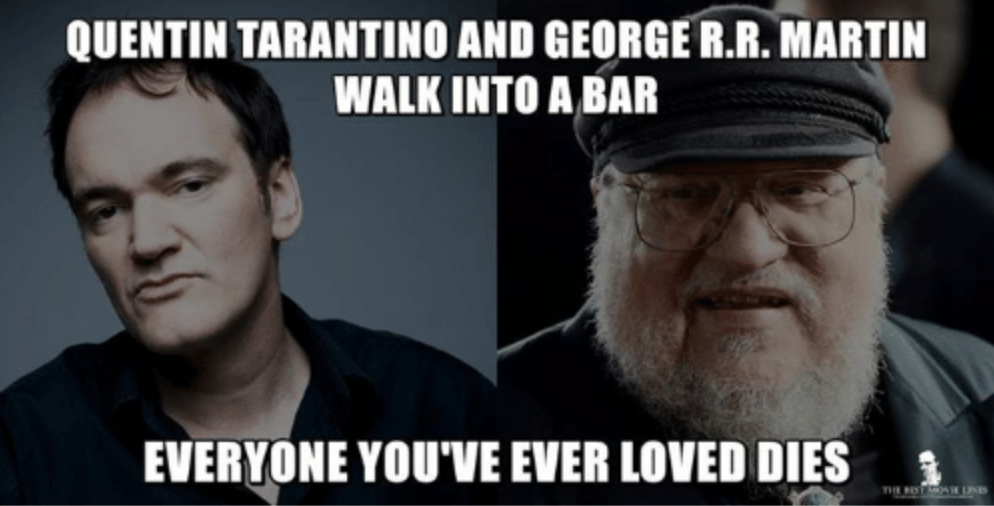
\includegraphics[width=\linewidth]{Tarantino}
	\end{subfigure}%\hskip 1em%
	\begin{subfigure}[t]{0.45\textwidth}
		\caption{}
		\centering
		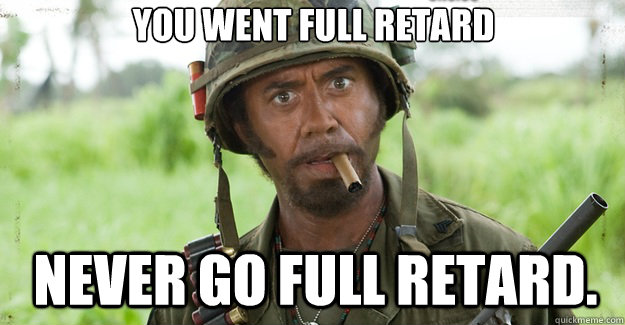
\includegraphics[width=\linewidth]{fullretard.jpg}
	\end{subfigure}
	\label{phd-crsi}
	\caption*{Fonte: autor}
\end{figure}

\begin{table}
	\centering
	\caption{Exemplo do pacote \textit{adjustbox} (que coloca o comprimento da tabela igual ao do texto, isso é muito útil!). Note que é necessário usar o \textit{top, mid e bottomrule} para diferenciar a espessura das linhas}
	\begin{adjustbox}{max width=\textwidth}
		\begin{tabular}{c|ccccc}
			& Composição& Símbolo de &Grupo &Designação & \\
			Fase &\%at. Si & \textit{Pearson} &espacial &\textit{Strukturbericht} &Protótipo \\
			\toprule
			(Cr) & 0 a 9,5 & $cI2$ & $Im-3m$& $A2$&W\\
			\hline
			(Si) & \~ 100 & $cF8$ & $Fd-3m$ & $A4$ & C (diamante) \\ 
			\hline
			Cr$_3$Si & 22,5 a 26,4 & $cP8$ & $Pm-3n$ & $A15$ & Cr$_3$Si\\
			\hline
			$\alpha$-Cr$_5$Si$_3$ & 36 a 41 & $tI32$ & $I4/mcm$& $D8_m$ & W$_5$Si$_3$\\
			\hline
			$\beta$-Cr$_5$Si$_3$ & --- & --- & --- & --- & --- \\
			\hline
			CrSi & 50 & $cP8$ & $P2_13$ & $B20$ & FeSi\\
			\hline
			CrSi$_2$ & 66,7 a 67 & $hP9$ & $P6_222$ & $C40$ & CrSi$_2$\\
			\bottomrule
		\end{tabular}
	\end{adjustbox}
	\label{tab:estruturas-cristalinas-Cr--Si}
	\caption*{Fonte: autor}
	\caption*{Nota: adaptado de \cite{Gokhale1987}}
\end{table}

Exemplo de itens:

\begin{enumerate}
	\item Texto 1
	\item Texto 2
	\item Texto 3
\end{enumerate}



% ----------------------------------------------------------
\chapter{Revisão bibliográfica}

\section{Seção 1}

\section{Seção 2}

\section{Seção 3}


% ----------------------------------------------------------
% ----------------------------------------------------------
\chapter{Materiais e métodos}

\section{Seção 1}

\subsection{Subseção 1}

\subsubsection{Subsubseção 1}


\chapter{Resultados e discussão}


%--------------------------------------------------------
\chapter{Conclusões}


%

\postextual

\bibliography{Cr-Si-B.bib}
%Deve-se criar um arquivo \textit{.bib} 

\chapter*{Anexos}
\label{anexo:refinamentos}
\addcontentsline{toc}{chapter}{ANEXOS}
%Adiciona o capítulo ANEXOS ao sumário

\renewcommand\thesection{A}
%Ao invés de colocar no sumário em números, este renewcommand coloca como A, ou B, ou C... Tem que mudar manualmente!

\section{Código Python para conversão de bases}
\label{Python-Conversão de bases}

O pacote \textit{verbatim} configura tudo como texto corrido.

\begin{verbatim}

#Pacotes do python.
import numpy as np
import numpy.linalg as la

#Define uma lista alat extraindo os valores do arquivo de entrada.
alat = np.genfromtxt('atomic-positions-alat.txt')

#Define as bases.
b1 = np.array([[1.,0.,0.],[0.,1.,0.],[0.,0.,1]]) # alat
b2 = .5 * np.array( [ [1.,-1.,1.], [1.,1.,1.], [-1.,-1.,1.] ] ) 
# crystal, ibrav=7

#Operação de matrizes.
M1 = np.transpose(b1)
M2 = np.transpose(b2)
M2inv = la.inv(M2)

#Cálculo da mudança de base.
T = np.dot(M2inv,M1)

#Cria uma matriz de zeros 3x3.
crystal = np.zeros([len(alat),3])

#Adiciona os valores convertidos a lista crystal após a mudança de base.
for i in range(len(alat)):
crystal[i] = (np.dot(T, alat[i]))
print "%21.9ft%12.9ft\%12.9f" % (crystal[i,0], crystal[i,1], crystal[i,2])
\end{verbatim}

\end{document}
